
%======================问题介绍====================================
\section{Introduction}
According to the statistical data collected by World Heath Organization(WHO)[cite], the current Ebola virus disease (EVD) outbreak ravaging three nations in West Africa has affected more than 14,000 persons and killed over 5,000. It is the longest and most widely spread Ebola epidemic ever seen. In this problem, a new medication has just been released by the world medical association. We are required to undertake the duty of fight against the Azrael with the aid of this medicine: establish a realistic sensible and useful model that consider various factors including spread speed, medicine manufacturing speed, delivery system, etc. In order to accomplish such a huge task, we establish two sub-models:
\begin{itemize}
\item \textbf{Sub-model 1:} Model which describes the virus dispersal process in ideal settings.
\item \textbf{Sub-model 2:} Model contains the deep relationship between the medication manufacturing, delivery, applying flow and the infection, immune process of EVD. 
\end{itemize} 
In sub-model 1, we implement a real-time simulation system by Matlab to simulate the dispersal process of Ebola in ideal cases. We modify the SIR model into our SID one and exhibit you with touchable and vivid figures.
In sub-model 2, by surveying a large amount of data, scientific paper available, we propose an all new model: \textbf{SPARD}, which takes not only: spread speed, harmfulness, delivery system, but also: manufacturing speed, dispersal path as essential factors. In addition, all these factors in \textbf{SPARD} model are dynamic changing and they provide us with a warning system which can aid us finding the trend of EVD dispersal as soon as possible.
The structure of the paper is organized by two sub-models, respectively. In each sub-model, we give our own assumptions, models descriptions, experiment results and strengths/weaknesses analysis. The final conclusion is given in section 4. The informal letter and some important codes are shown in Appendix. 

\section{Sub-model 1: The dispersal of the Azrael in ideal cases}
\subsection{Symbols and Notations}
\begin{table}[htbp]
\centering
\caption{Symbol and Notation list for sub-model 1}
 % Table generated by Excel2LaTeX from sheet 'Sheet1'
\begin{tabular}{|c|c|c|c|c|c|c|}
\hline
                                      \multicolumn{ 7}{|c|}{{\bf Symbols and Notations}} \\
\hline
\multicolumn{ 2}{|c|}{{\bf Symbol/Notation}} &                  \multicolumn{ 5}{|c|}{{\bf Physical Meaning}} \\
\hline
\multicolumn{ 2}{|c|}{$\tau$} & \multicolumn{ 5}{|c|}{The transmission probability from susceptible to infective} \\
\hline
\multicolumn{ 2}{|c|}{$\mu$} & \multicolumn{ 5}{|c|}{The transmission probability from infective to death} \\
\hline
\multicolumn{ 2}{|c|}{$S(t)$} & \multicolumn{ 5}{|c|}{The number of susceptible people at time t} \\
\hline
\multicolumn{ 2}{|c|}{$I(t)$} & \multicolumn{ 5}{|c|}{The number of infected people at time t} \\
\hline
\multicolumn{ 2}{|c|}{$D(t)$} &     \multicolumn{ 5}{|c|}{The number of dead people at time t} \\
\hline
\multicolumn{ 2}{|c|}{N} & \multicolumn{ 5}{|c|}{The total population in one district(default: 1 unit)} \\
\hline
\multicolumn{ 2}{|c|}{$t_{max}$} &                 \multicolumn{ 5}{|c|}{Maximum simulation days} \\
\hline
\multicolumn{ 2}{|c|}{$k$} &    \multicolumn{ 5}{|c|}{Average days to death after infected} \\
\hline
\end{tabular}  

\end{table}
\subsection{Analysis and Assumptions}
In this section, our goal is to construct a model which can provide us with a direct and visible Ebola spread process in those highlighted areas, specifically without any sanitation interference. The goal for conducting such an experiment is to set up a fundamental pipeline for further models, which introduced in the following two sections. According to the official document, Guidance for Immunization Programmes in the African Region[cite], released in Oct. 2014, at the present EVD outbreak, the top three countries in EVD crisis, which means they own the most detected cases and fatality rates, are \textit{Guinea, Liberia and Sierra Leone}. Besides, \textit{Cote d' Ivorie, Guinea Bissau, Mali} and another eleven countries are in high infection risk. Just as we shown in \textbf{figure 1}, those countries are mostly in Western African regions.
In addition, according to another technical report[cite] the common approach of EVD's spread are: human direct contacts, body fluids exchanges, etc. One of the issues worthy noting is that no evidence yet attests that there exists human-stock dispersal path or ocean movement path. In other words, the spread of EVD major rely on high population density and commence from those relative inner parts of the continent. This implies that our EVD dispersal spread point in the simulation should be set in metropolitans. 
\begin{figure}[htbp]
\centering
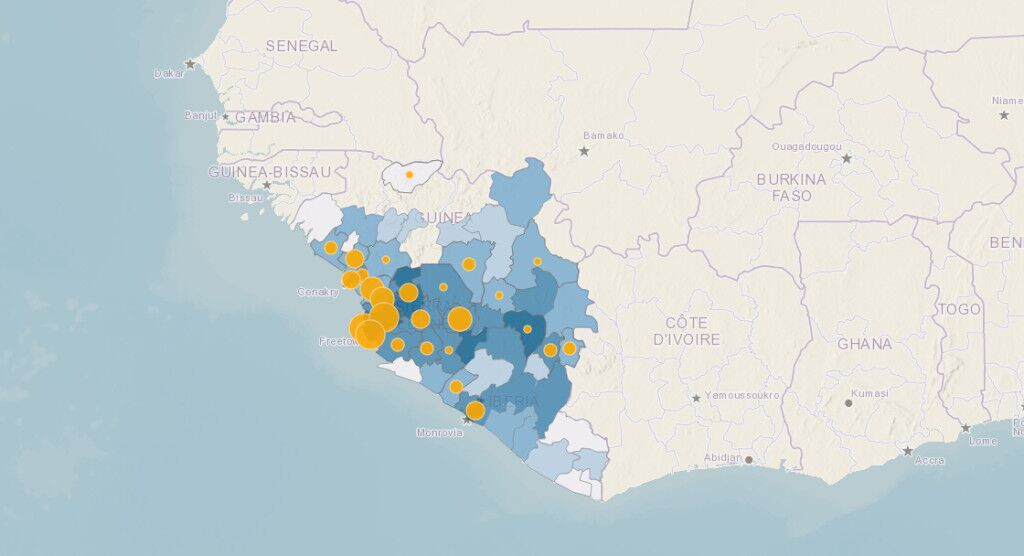
\includegraphics[width=15cm]{/figure/fig1.jpg}
\caption{The present status of Ebola in Western African areas, according to WHO website} \label{fig:1}
\end{figure}
Besides, in order to direct observe the disastrous effect of Ebola and utilize the classical SIR model, we survey the Ebola's infection probability for a given patient from [cite]. For simplification purpose, we utilize the "max-pooling" strategy to select our infectious probability $\tau$. And because we assume there does not exist any health or medication care system, we set the death rate$\mu$ as $100\%$ for those infected people. Finally, because the incubation period for an EVD patient ranges from 2-21 days[cite], we suppose that the life-span only depends on its average value.

On the basis of the analysis above, we summarize our assumptions as below:
\begin{itemize}
\item \textbf{Assumption 1-1:} The starting points of the dispersal should be cities selected at random rather than other points on the map.
\item \textbf{Assumption 1-2:} There is not any human medical-care actions to infect or stop Ebola's spread. As long as someone is infected by EVD, he or she is bounded to death, $\mu=100\%$.
\item\textbf{Assumption 1-3:} The dispersal approach only includes continent-adjacent dispersal approach.
\item\textbf{Assumption 1-4:} The lifespan for a infected people $k$ is a constant depending on the incubation period.
\end{itemize} 
\subsection{Model Description}
In this subsection, we briefly introduce the classical \textbf{S}usceptible, \textbf{I}nfective, \textbf{R}emoval(\textbf{SIR}) model[cite] in epidemic dynamic fields and our modification work on it. Besides, we will introduce both of the input parameters and output ones and the basic flow of our simulation system.
First and foremost, according to the SIR model, as long as a particular region is affected by the Ebola, the whole population can be divided into three separate parts: \textbf{S}usceptible(People who are still in healthy status); \textbf{I}nfective(People who has already caught the EVD); \textbf{R}emoval(\textbf{SIR})(People who has already recovered and is immune to EVD). Nonetheless, on the basis on \textbf{Assumption 1-2}, there should not be any recovered people. When we recall the fact that no matter recovered or death people are immune to the disease and are not able to further affect susceptible guys. We can simply consider that "Removal" is equivalent to "Death"; therfore, we modify SIR into SID(death) by set D's immune index at 0(because they have already died). The core of the SIR model also includes two transmission probability: susceptible-infective $\tau$ and infective-removal(death)$\mu$. Based on the early assumptions, $\mu$ has already selected at $100\%$. In order to calculate susceptible-infective transmission probability $\tau$, we utilize the apex value in [cite], just as shown in \textbf{figure 2}. Therefore, we set $\tau$ at $0.4$. 
\begin{figure}[htbp]
\centering
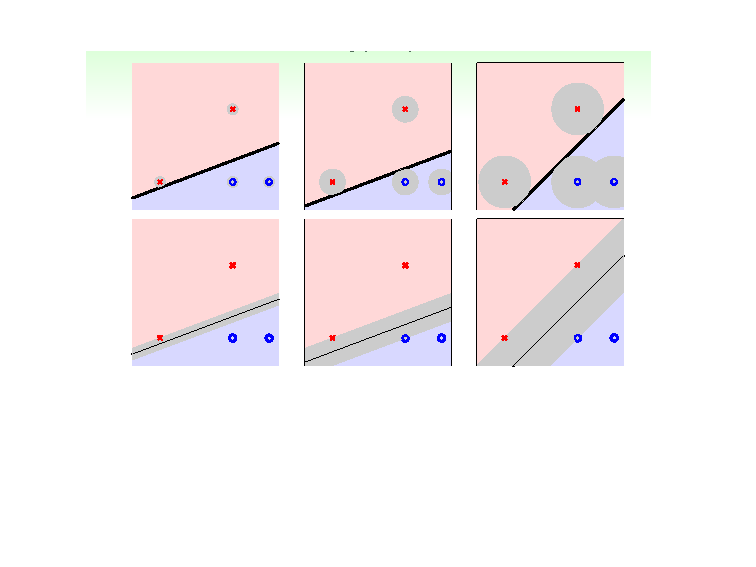
\includegraphics[width=15cm]{/figure/fig2.pdf}
\caption{The probability of infecting suspicible people of an EVD patient, with respect to time}\label{fig:2}
\end{figure}
According to \textbf{Assumption 1-4}, the lifespan for infected people $k=13 days$. The purpose of SID model is to model the S, I, D kinds of people with a group of differential equations as below:
\begin{equation}
 \left\{
\begin{aligned}
S\left( t\right) +I\left( t\right) +D\left( t\right) =N \\
\dfrac {dS}{dt}=-\tau SI \\
\dfrac {dI}{dt}=\tau SI-I\mu \\
\dfrac {dD}{dt}=I\mu \\
S(0)=N, I(0)=0, D(0)=0
\end{aligned}
\right.
\end{equation}
Note that $N$ is the total population of a specific district; at the initial state, all the people in one district is uninfected by EVD, and of course, there is no death. Thus, we set the initial value of the differential equation groups at $S(0)=N, I(0)=0, D(0)=0$.

The second task of this model is to determine other essential rules and parameters for our simulation system. Due to \textbf{Assumption 1-1}, we set the dispersal rule "four-adjacent" principle respecting to the pixels on the map,i.e., if one particular pixel is set as infected at day $n$, its four neighbour pixels(upper, lower, left and right one) have probability $\tau$ to be affected. Moreover, for the sake of observing the dynamic process of EVD's spread, we trace $t_max=120days$ to generating the simulation results. The evaluation metric is the relative ratio of S, I and D. Another interesting issue is to determine the starting cities of EVD in the simulation. \textbf{Assumption 1-1} and the characteristic of Ebola hint us to select those cities with large population and relatively lower hygiene level. Therefore, we survey those potential cities with high EVD risk(including population, countries' hygiene level:hospital beds, physician numbers) and eventually select four cities, according to the WHO 2014 annual report[cite]. Our investigation result about those cities is shown in \textbf{table 2}.
\begin{table}[htbp]
\centering
\caption{The survey result of four selected cities}
% Table generated by Excel2LaTeX from sheet 'Sheet1'
\begin{tabular}{|r|r|r|r|r|}
\hline
{\bf city} & {\bf country} & {\bf city population} & {\bf hospital beds\tnote{1}} & {\bf physician number\tnote{2}} \\
% city &  country &  city population & hospital beds\tnote{1} &  physician number \\
\hline
   Korhogo & Côte d'Ivoire &     174000 &        1.7 &        1.4 \\
\hline
    Kankan &     Guinea &     193830 &        1.2 &        0.9 \\
\hline
    Bamako &       Mali &    1800000 &        0.8 &          1 \\
\hline
    Tamale &      Ghana &     562919 &          1 &          2 \\
\hline
\end{tabular}  
\begin{tablenotes}
        \footnotesize
        \item[1] hospital beds and physician number are in 10,000 population scale.
\end{tablenotes}

\end{table}


\subsection{Experiment Result}
In this subsection, we exhibit the automatic simulation results of EVD in ideal cases. In \textbf{figure 3}, we show the relative SID changing curve respect to time:
\begin{figure}[htbp]
\centering
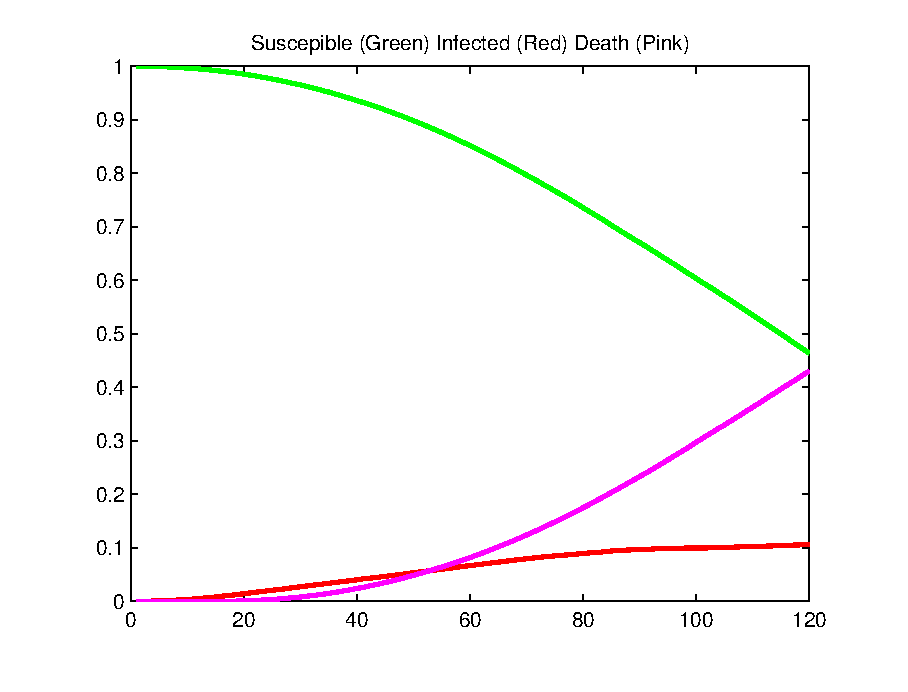
\includegraphics[width=15cm]{/figure/fig3.eps}
\caption{The S,I and D relative changing curve with respect to time}\label{fig:3}
\end{figure}
From the simulation figure, we can observe that the susceptible and death curve are changing exponentially. If we choose 80\% as the threshold of susceptible, a commonly used index to indicate the harmfulness of one particular pestilence, the milestone happens approximately on the 60th day. The counterpart index of SARS is 64th day[cite]. Besides, in the light of the end part of the curve, we can predict that the percentage of death will exceed the percentage of susceptible in the following few days, which means the comprehensive collapse in this area. These facts notifies us that the Ebola is indeed a lethal disease with high infectious rate.
In \textbf{figure 4}, we visualize the dispersal process by sampling four days simulation result.
\begin{figure}[htbp]
\centering
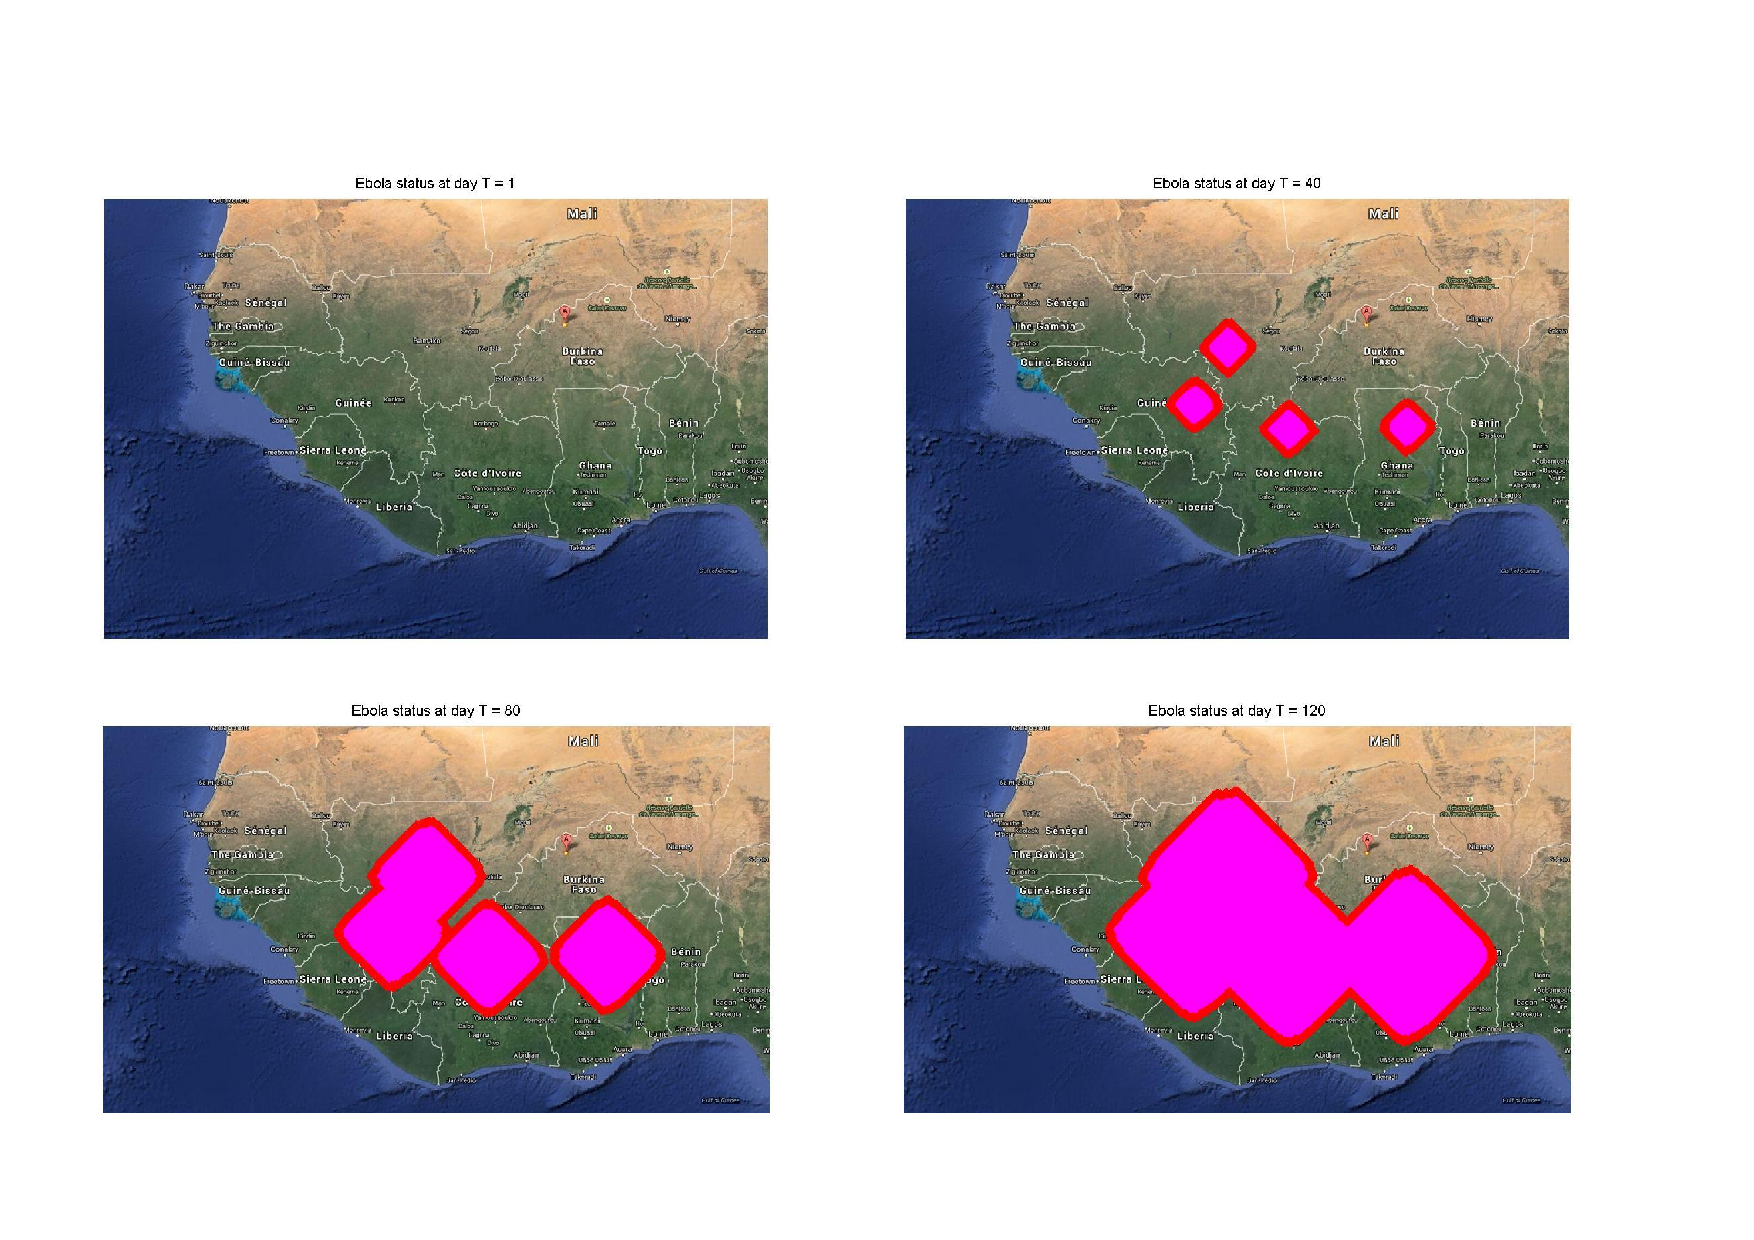
\includegraphics[width=12cm]{/figure/fig4.pdf}
\caption{A dynamic dispersial process of EVD by sampling 1st day, 40th day, 80thday and 120th day}\label{fig:4}
\end{figure}
In \textbf{figure 4}, the continent parts with original color are uninfected areas(the S area); the pink parts are those districts which have already in collapse condition(the D area); the red outer skirt of the pink parts are districts where are suffering from the EVD(the I area). \textbf{Figure 4} inspire us at least in two aspects: 1. the dispersal of Ebola in ideal cases is a diamond-shape infiltration process(this can help us to predict risky districts); 2. As long as several infection districts are connected together, the red outer skirt will dramatically decrease, which means acute increase in death(therefore, we should stop this circumstance from happening).
\subsection{Strengths and Weaknesses}
\begin{itemize}
  \item Strenghs
  \begin{itemize}
    \item We successfully model the dispersal process of Ebola by revising the classical SIR model into SID model and by setting reality parameters to it.
    \item By utilizing the simulation system, there is no need to achieve the numerical solution to the differential equations in SID model.
    \item The simulation system enables us to visualize the process of dispersal in a direct and understandable way.
  \end{itemize}
  \item Weaknesses
  \begin{itemize}
    \item The primary model fails to evaluate some crucial factors which can affect the spread, for instance, there should be a relationship between the population density and the infection probability $\tau$ in a specific region.
    \item The simulation process itself may take a considerable time. We spend over three minutes to fetch the results on a Core-i5 PC with 8GB RAM. In fact, both of the time and space consumptions are $O(mapSize*t_{max})$.
  \end{itemize}
\end{itemize}

\section{Sub-model 2: Improved EVD dynamic dispersal model}
\subsection{Symbols and Notations}
\begin{table}[htbp]
\caption{Symbol and Notation list for sub-model 2}
\center
% Table generated by Excel2LaTeX from sheet 'Sheet1'
\begin{tabular}{|cc|ccccc|}
\hline
                                      \multicolumn{ 7}{|c|}{{\bf Symbols and Notations}} \\
\hline
\multicolumn{ 2}{|c|}{{\bf Symbol/Notation}} &                  \multicolumn{ 5}{|c|}{{\bf Physical Meaning}} \\
\hline
\multicolumn{ 2}{|c|}{$S(x,y,t)$} & \multicolumn{ 5}{|c|}{The number of susceptible people at time t} \\
\hline
\multicolumn{ 2}{|c|}{$P(x,y,t)$} & \multicolumn{ 5}{|c|}{The number of primary infected people at time t} \\
\hline
\multicolumn{ 2}{|c|}{$A(x,y,t)$} & \multicolumn{ 5}{|c|}{The number of advanced infected people at time t} \\
\hline
\multicolumn{ 2}{|c|}{$R(x,y,t)$} & \multicolumn{ 5}{|c|}{The number of recovered people at time t} \\
\hline
\multicolumn{ 2}{|c}{$D(x,y,t)$} &      \multicolumn{ 5}{|c|}{The number of dead people at time t} \\
\hline
\multicolumn{ 2}{|c|}{$N(x,y,t)$} & \multicolumn{ 5}{|c|}{The total population in one district(default: 1 unit)} \\
\hline
\multicolumn{ 2}{|c|}{$\tau(x,y,t)$} & \multicolumn{ 5}{|c|}{The transmission probability from susceptible to primary infected} \\
\hline
\multicolumn{ 2}{|c|}{$\mu(x,y,t)$} & \multicolumn{ 5}{|c|}{The transmission probability from advanced infected to death} \\
\hline
\multicolumn{ 2}{|c|}{$\lambda(x,y,t)$} & \multicolumn{ 5}{|c|}{The transmission probability from primary infected to recovery} \\
\hline
\multicolumn{ 2}{|c|}{$\pi(x,y,t)$} & \multicolumn{ 5}{|c|}{The transmission probability of immuning} \\
\hline
\multicolumn{ 2}{|c|}{$\phi(x,y,t)$} & \multicolumn{ 5}{|c|}{The transmission probability from primary infected to advanced} \\
\hline
\multicolumn{ 2}{|c|}{$t_{max}$} &                 \multicolumn{ 5}{|c|}{Maximum simulation days} \\
\hline
\end{tabular}  
\end{table}
\subsection{Analysis and Assumptions}
In this section, we concentrate our attention to further revising the simple SID model mentioned in the former section and improving our accuracy and performance of our own model. Our contributions can be classified into three fields:
\begin{itemize}
  \item The residents in one particular district $(x,y)$ at time $t$ is detailed divided into five classes susceptible, primary infected, advanced infected, recovered and immune, death. All these values are variables with respect to spatial and temporal.
  \item We succeed in establishing a numerical relationship between transmission probabilities from five classes above. The probabilities themselves are also in dynamic status corresponding to time and geography location.
  \item We succeed in establishing the demand of the medication at $(x,y,t)$. And construct an "\textbf{E}arly \textbf{W}arning \textbf{S}ystem(\textbf{EWS})" for vaccine medicine.
  \item In the aspect of delivery system, we take the advantage of graph optimization technique to implement a medication delivering optimized arrangement based on the dynamic actual demands.
 \end{itemize}
 The general human classification and their transmission probabilities is shown in \textbf{figure 5}. For abbreviation purpose, we name our model as \textbf{S}usceptible, \textbf{P}rimary, \textbf{A}dvanced, \textbf{R}ecovery, \textbf{D}eath(\textbf{SPARD}).
\begin{figure}[htbp]
\centering
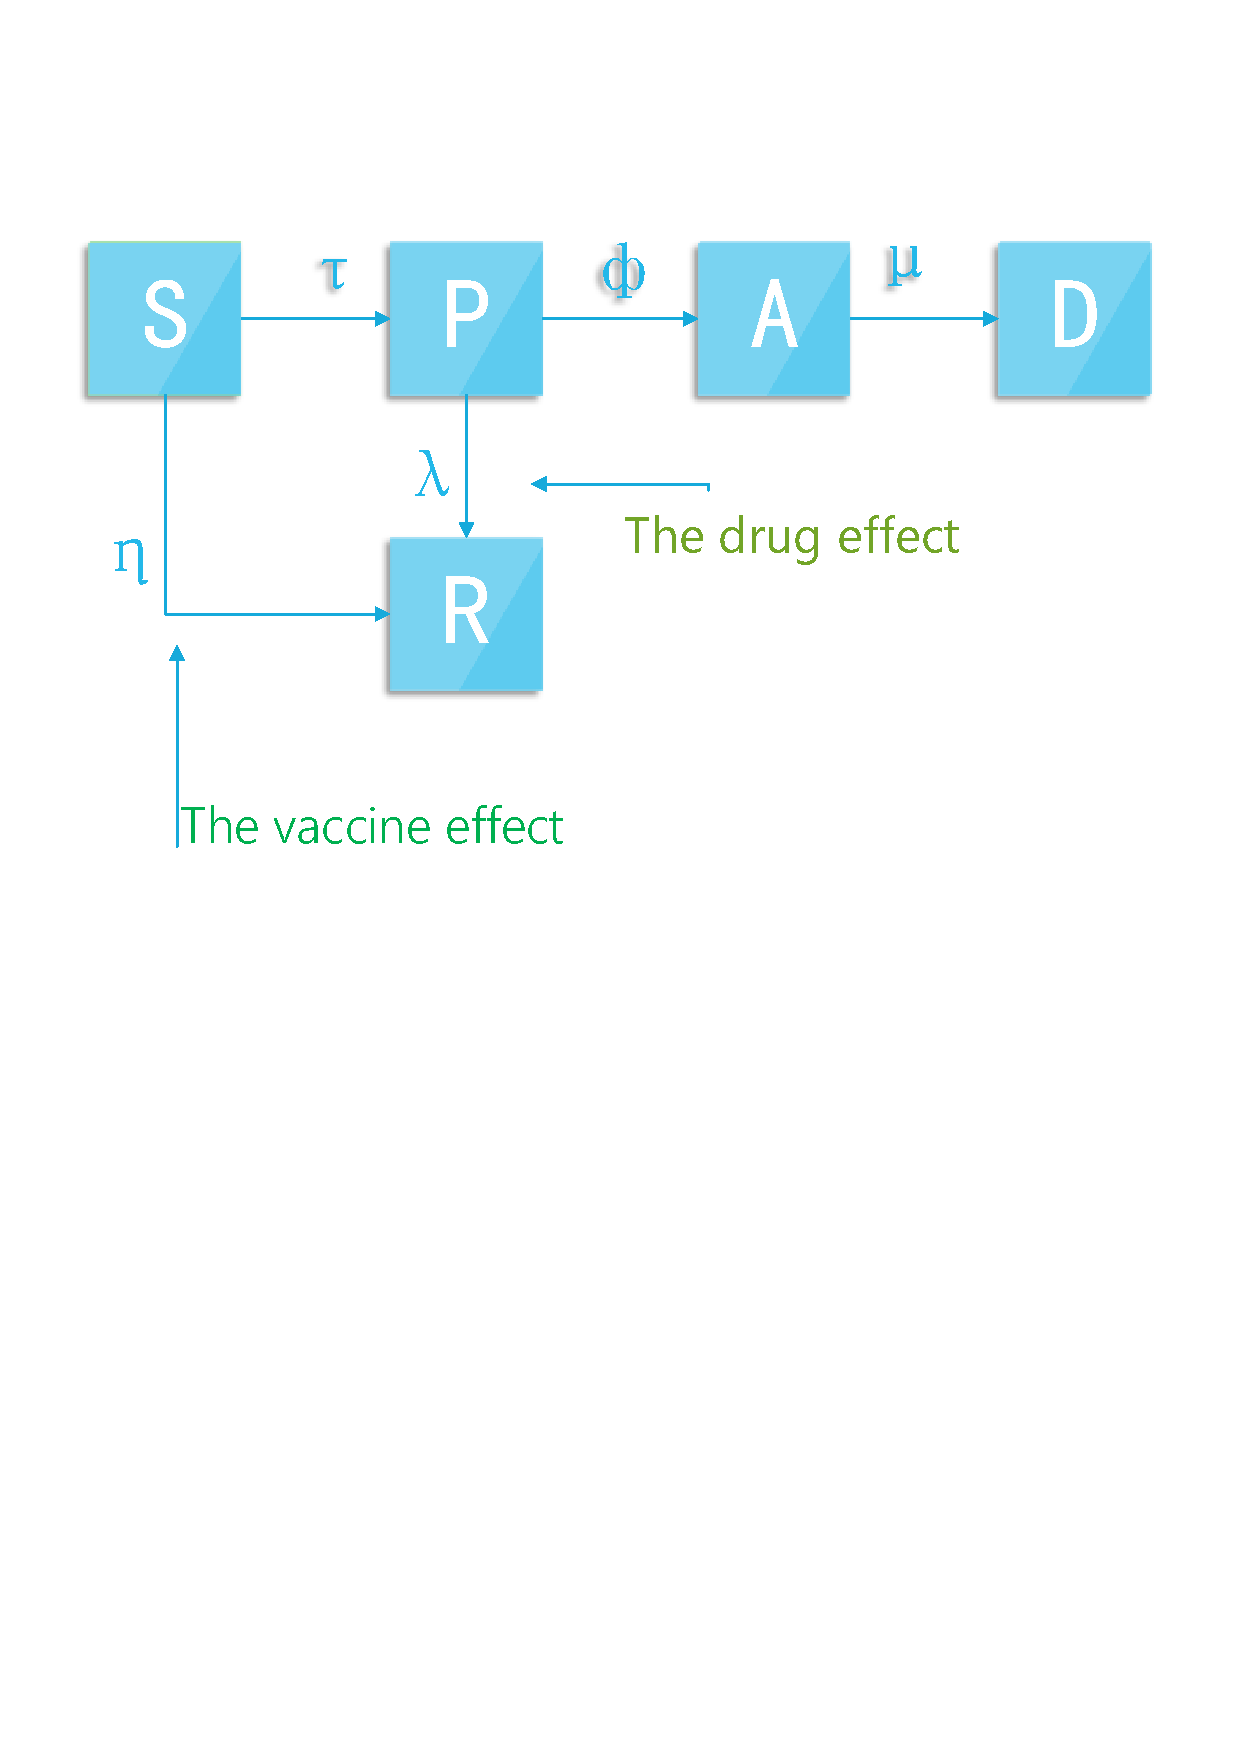
\includegraphics[width=12cm]{/figure/fig5.pdf}
\caption{The flow chart of our proposed SPARD dispersal model for EVD}\label{fig:5}
\end{figure}
Our definition of "Susceptible", "Death" is as same as those in section 2: the primary SID model in ideal cases. What needs to be specially explained is: "Primary" status, people which have determined to have infected by EVD but still in primary stage. In other words, this kind of people are treatable with the aid of our newly invented medication with probability $\lambda$. The counterpart of "P" status is the "A": advanced infected status. People in this stage are unfortunately incurable by our medicine(because the problem says that the medicine is only valid to early stage people) and they are bounded to death at a constant rate. The transition probability from "P" stage to "A" stage is $\phi$. Moreover, thanks to the invention of vaccine by the world medication organization, people in susceptible status are able to become permanent immune to EVD(the "R" status) with probability $\eta$. 
Besides in order to further simulate and analysis this model numerically , we put out following model assumptions. Note that some of them will be explained in detail in next subsection.
\begin{itemize}
\item \textbf{Assumption 2-1} There is no possibility of natural recovery for any EVD patient, no matter a primary stage one or an advanced stage one.
\item \textbf{Assumption 2-2} The effect of EVD dispersal at a specific point to its neighbourhood is a circle with constant radius, which modulated by a function. 
\item \textbf{Assumption 2-3} The dispersal abilities of "P" and "A" status patients are different constants.
\item \textbf{Assumption 2-4} A "P" status patient usually with slight symptoms and is taken care by five families members(on average) every day. A "A" status patient is looked after by one professional medical staff(on average) during rest lifespan.
\item \textbf{Assumption 2-5} The medical level and people's awareness to EVD is a monotonous increase function with respect to time.[cite]
\item \textbf{Assumption 2-6} The average delivery period of both vaccine and remedial drug is a constant.
\end{itemize} 

\subsection{Model Description}
\subsubsection{General Model}
We get inspired from our primary sub-model 1 and [cite]. The overall EVD dispersal system in district $(x,y)$ at time $t$ is still described by differential equation group as below:

\begin{equation}
 \left\{
\begin{aligned}
 S\left( x,y,t+1\right) =\left( 1-\tau -\eta \right) S\left( x,y,t\right) \\
 P\left( x,y,t+1\right) =(1-\phi-\lambda)p\left( x,y,t\right) +\tau S\left( x,y,t\right) \\
 A\left( x,y,t+1\right) =\left( 1-\mu \right) A\left( x,y,t\right) +\varphi P\left( x,y,t\right) \\
D\left( x,y,t+1\right) =D\left( x,y,t\right) +\mu A\left( x,y,t\right) \\
R\left( x,y,t+1\right) =R\left(x,y,t\right)+\lambda P\left( x,y,t\right) +\eta S\left( x,y,t\right) \\
\end{aligned}
\right.
\end{equation}
The differential equation group above describe the dynamic transition process from time $t$ to time $t+1$. Nonetheless, as mentioned in last subsection, in SPARD, the transition probabilities are also dynamic. In other words, their values depend on the present status of a local point. From 3.3.2 to 3.3.7, we explain our transition models, respectively. In 3.3.8, we will introduce our \textbf{E}arly \textbf{W}arning \textbf{S}ystem(\textbf{EWS}) in detail. Section 3.3.9 is another graph model concerning transport optimization issue.
\subsubsection{Objective Condition Model}
According to the guide released by WHO to fight against EVD[cite], it is highlighted that the hygiene infrastructure level, including hospital beds, laboratories and surveillance ability, along with local people's awareness to EVD, play crucial roles in eradicating Ebola. In our SPARD model, we generally classify those factors as "Objective Conditions". As far as we are concerned, those objective conditions can be considered as an monotonous increase function to time, which means that the overall hygiene level and human beings knowledge is turning better daily(textbf{Assumption 2-5}). To exemplifier this idea, we collect NGO volunteer number(data from [cite]) and Isolation beds(data from [cite]) in Liberia as crucial hygienic index provided by WHO from March, 2013 to December, 2014, as shown in \textbf{Table 4}. The visualized curve figure is shown in \textbf{figure 6}.
\begin{table}[htbp]
\centering
\caption{NGO volunteer number and EVD isolation beds in Liberia} 
% Table generated by Excel2LaTeX from sheet 'Sheet1'
\begin{tabular}{|c|c|c|}
\hline
{\bf Date \tnote{1}} & {\bf NGO Volunteer Number \tnote{2}} & {\bf Isolated Beds} \\
\hline
    Mar-13 &        287 &        2.3 \\
\hline
    Jun-13 &        296 &        2.6 \\
\hline
    Sep-13 &        311 &        3.1 \\
\hline
    Dec-13 &        363 &        3.4 \\
\hline
    Mar-14 &        533 &       3.41 \\
\hline
    Jun-14 &        611 &        3.7 \\
\hline
    Sep-14 &        642 &          4 \\
\hline
    Dec-14 &        684 &        4.2 \\
\hline
\end{tabular}  
\begin{tablenotes}
        \footnotesize
        \item[1] NGO volunteer number is collected on: http://www.arda.org
        \item[2] Isolated beds number is in 10,000 population scale. collected from: http://www.emergency.it 
\end{tablenotes}

\end{table}

\begin{figure}[htbp]
\centering
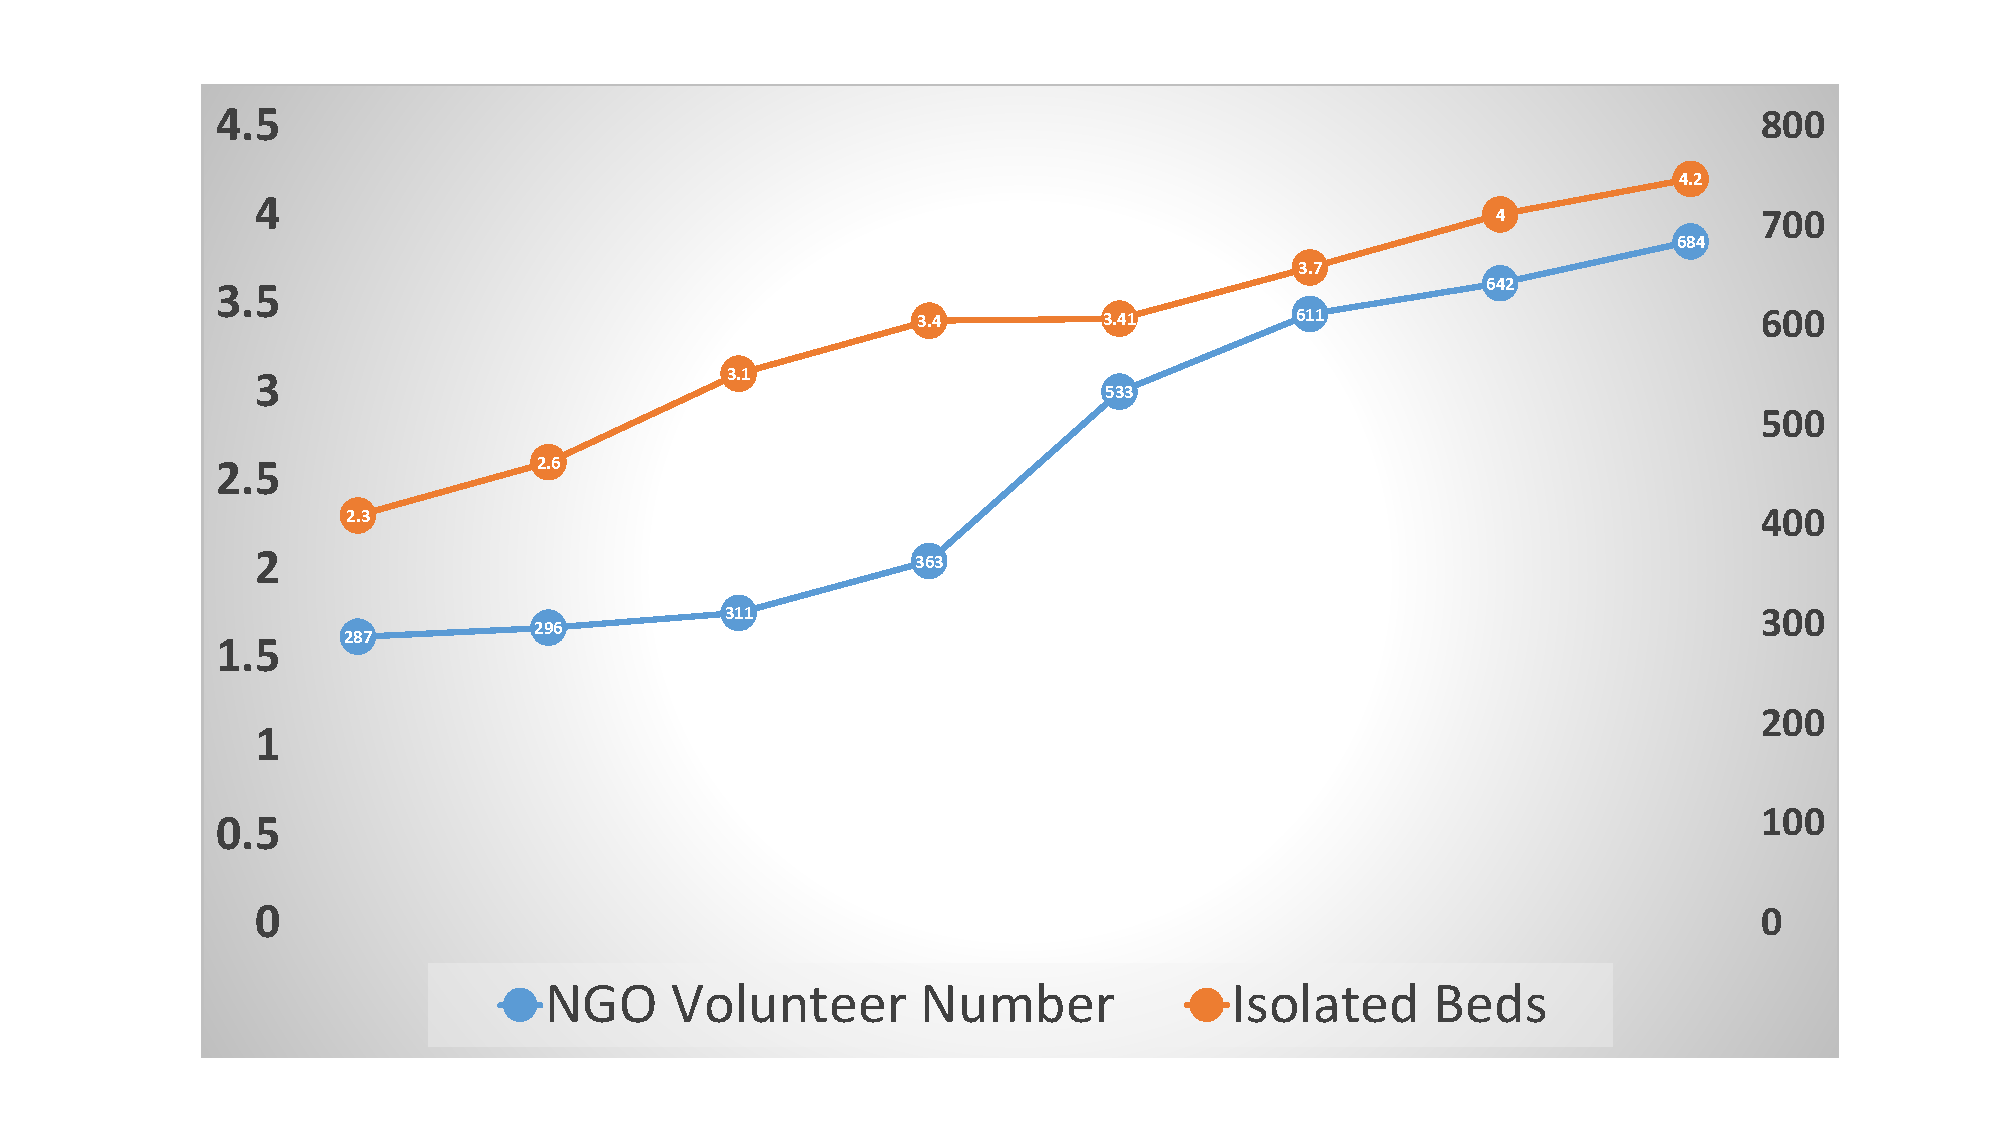
\includegraphics[width=12cm]{/figure/fig6.pdf}
\caption{The visualized changing curve of NGO volunteer number and isolated beds number from Mar, 2013 to Dec, 2014}\label{fig:6}
\end{figure}

From \textbf{figure 6}, we can find that both the volunteer number and the number of isolation ward have always been increase since March, 2013. In our opinion, the objective conditions level can be described with a logistic function[cite] in order to reflect the process of relieving the effect of EVD dispersal in some degree. Compare with \textbf{figure 6}, it is also reasonable to do so from the angle of functional fitting. Therefore, we define "Objective Condition Index" as below:
\begin{equation}
OCI\left( x,y,t\right) =\dfrac {a}{1+e^{-t}}
\end{equation}
What is amazing is that the shape logistic function fit the blue curve(NGO volunteer number) quite well! This function implies that the $OCI$ can be viewed as a "discount"(range from 0-1) over the transition probability between a slight case to a severe one(S-P, P-A, etc).

\subsubsection{S-P Transition Model}
As far as we are concerned, the susceptible-primary stage transition probability is the core attribute to describe the EVD dispersal dynamic process, because it requires us to consider lots of inherent status of the location, i.e., the ratio among S, P, A, R, D people. First, we define the potential average number of an Ebola patient(both P and A types) can spread his or her virus, as the District Dispersal Index: $DDI$:
\begin{equation}
DDI=\dfrac {S}{S+R}\left({P}\times 5\times 23\% +{A}\times 1\times 81\% \right)\times OCI(x,y,t+1)
\end{equation}
$\dfrac {S}{S+R}$ is the ratio in healthy people who can be infected by Ebola("S" people are not immune yet, whereas "R" ones are immune). Due to \textbf{Assumption 2-3}, we investigate the fact[cite] that, a "P" status patient has 23\% probability to spread disease to others; the same value of a "A" status one is 81\%. Moreover, according to \textbf{Assumption 2-4}, we add five(average families members number per "P" patient) and one(average medical staff number per "A" patient) to the inner product terms, respectively. 
Generally speaking, the $DDI$ tells us how many susceptible people can be infected in a particular district without considering inter-district spread cases under present situation.
In order to calculate the precise ratio of S-P transition probability, i.e., the $\tau(x,y,t+1)$, we need to take district $(x,y)$ neighbourhood into consideration. There is a fact that a relatively farther district $(x_{1},y_{1})$ has less dispersal impact on $(x,y)$ than a near one $(x_{2},y{2})$. We utilize a two dimension Gaussian function $Gau(x,y)$ to conduct a convolution integral with $DDI(x,y,t)$ on spatial scale:
\begin{equation}
 \left\{
\begin{aligned}
Gau\left( x,y\right) =\exp\left(-\left( \dfrac {x^{2}+y^{2}}{\sigma ^{2}}\right)\right)\\
\tau \left( x,y,t+1\right) =\textbf{conv}\left[ DDI\left( x,y,t\right) ,Gau\left( x,y\right) \right]\\
\end{aligned}
\right.
\end{equation}
Note that in $Gau(x,y)$, the deviation coefficient $\sigma$, is a parameter to control the degree of popular density at neighbourhood around district $(x,y)$: imaging that for those metropolitan, $\sigma$ should be relatively large, because they have much stronger EVD radiation ability. \textbf{Figure 7} shows our settings of $Gau(x,y)$ for metropolitan($\sigma=250$), and normal villages($\sigma=150$), respectively.
\begin{figure}[htbp]
\centering
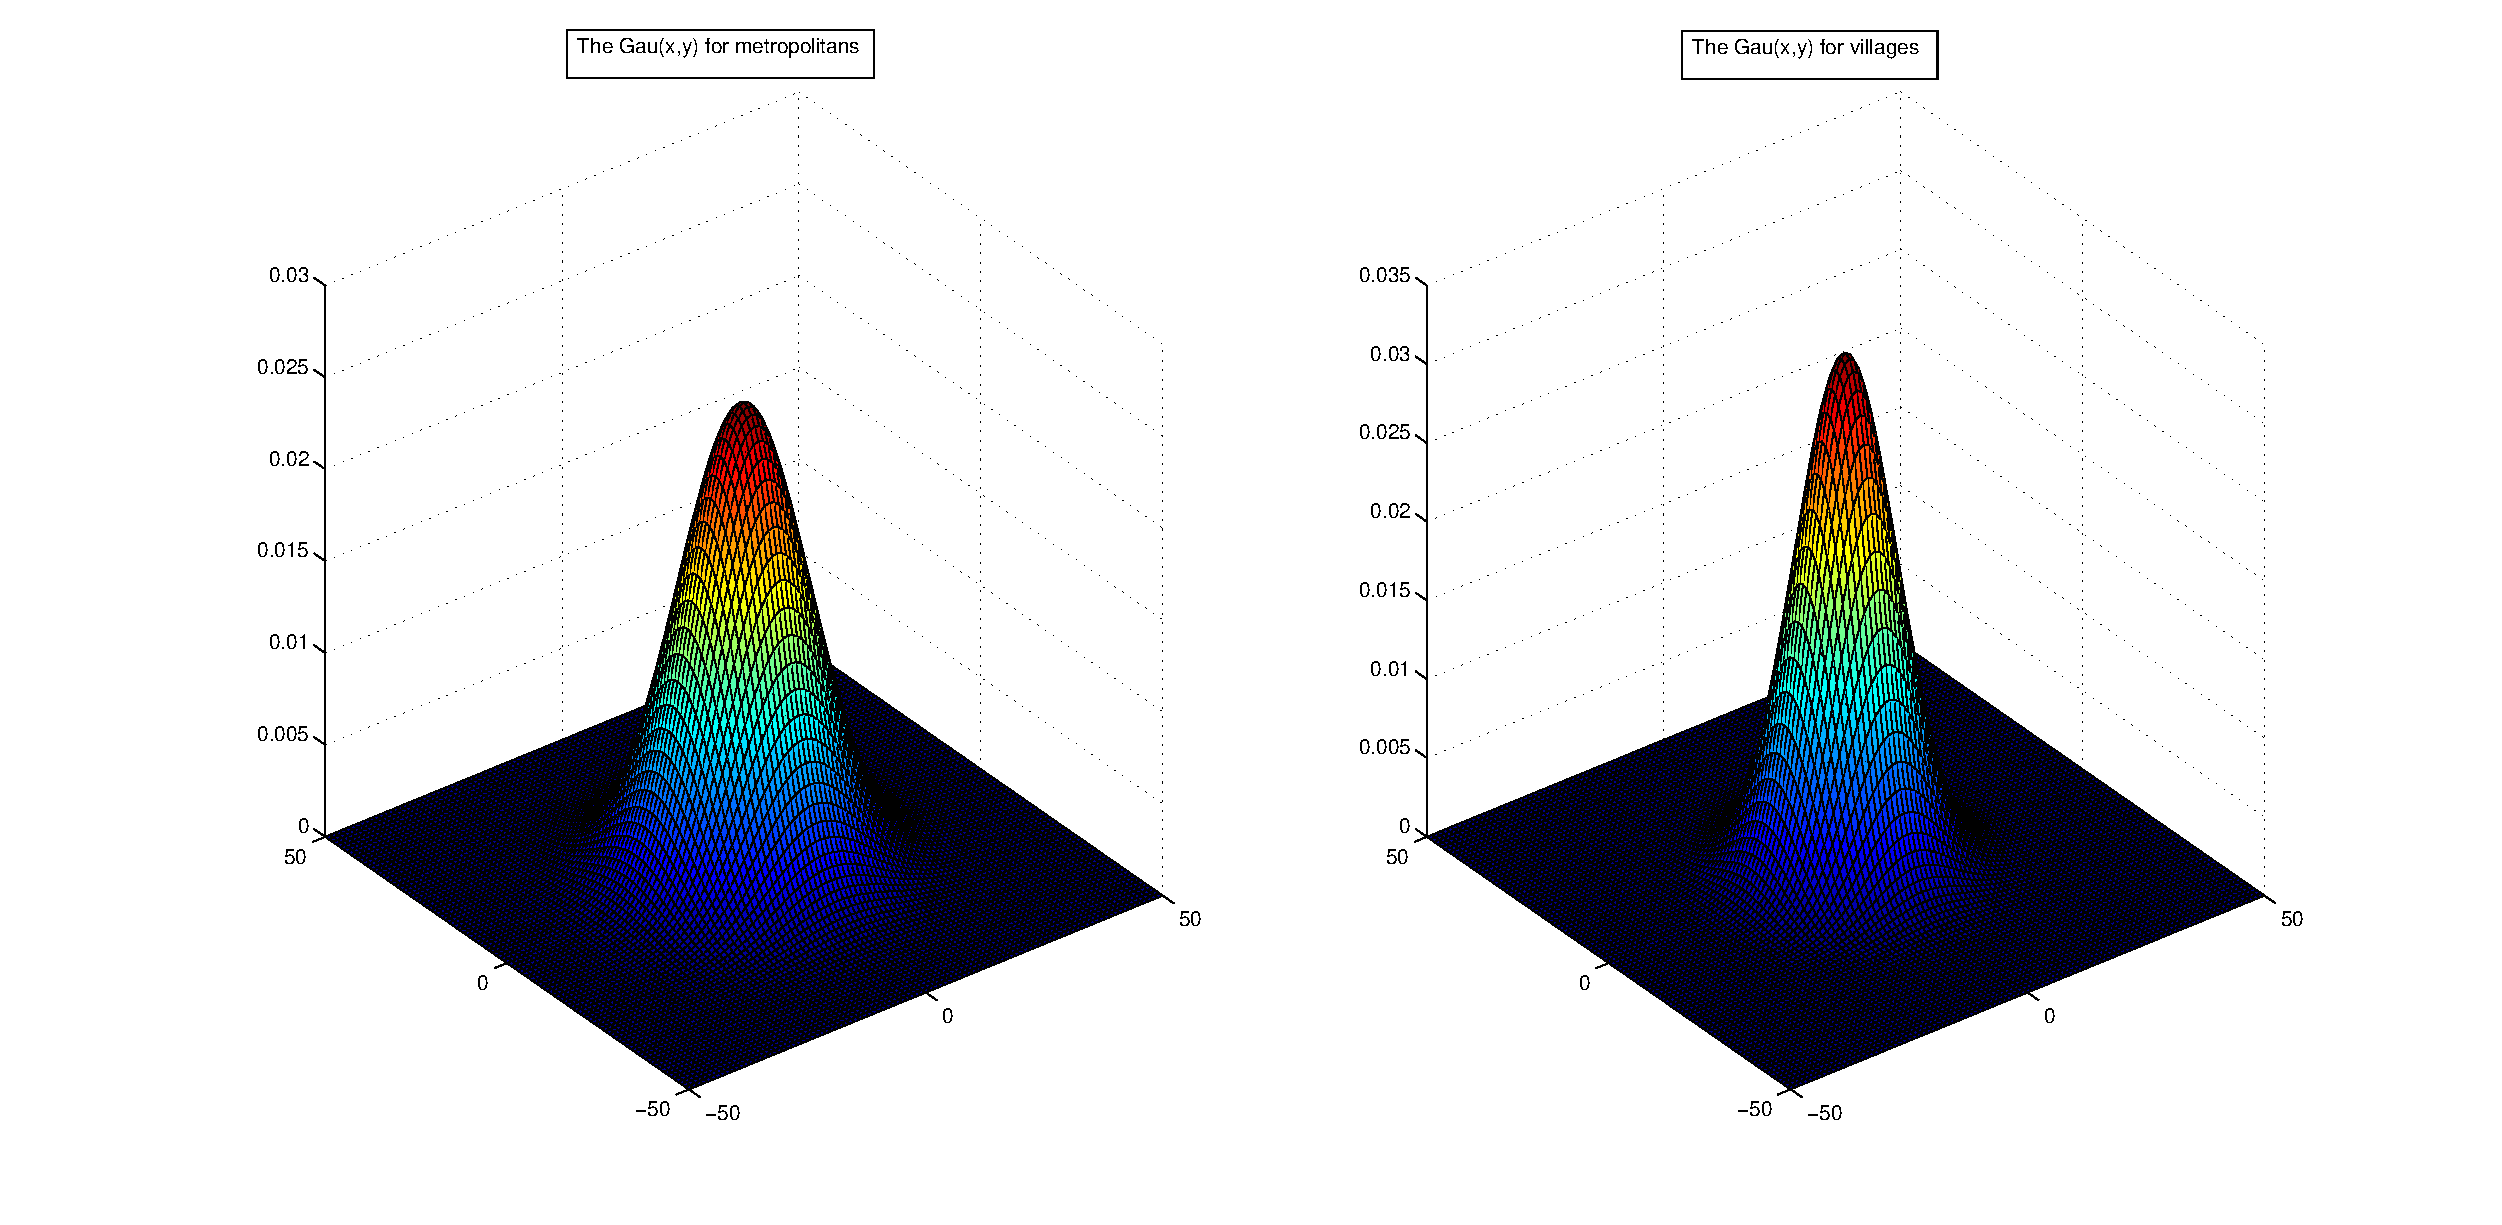
\includegraphics[width=15cm]{/figure/fig7.pdf}
\caption{The two dimension Gaussian function utilized to \textbf{conv} with DDI}\label{fig:7}
\end{figure}


\subsubsection{A-D Transition Model}
Unfortunately, the A-D transition ratio describes the process of advanced stage Ebola patient coming to death. In the light of an epidemic disease report[cite] and our own investigation of the severe symptoms of advanced stage EVD patients(including fever, rash, vomiting, bleeding, etc), we give \textbf{Assumption 2-1} which means that the advanced EVD patients have no possibilities to recover and die at a fixed rate every day. We set this ratio at $20\%$. Thus, we have $\mu=0.2$.  

\subsubsection{P-A Transition Model}
Thanks to the improvement in objective condition: the increase of $OCI$ with respect to time, we consider the transition probability from primary EVD to advanced EVD $\phi(x,y,t)$ a constant multiplied by the present $OCI$:
\begin{equation}
 \phi \left( x,y,t+1\right) =\phi \left( x,y,t\right) \times OCI(x,y,t+1)
\end{equation}

 \subsubsection{P-R Transition Model}
The P-R transition probability $\lambda$ means the ratio of people, who have caught Ebola with slight symptoms, be cured in a particular day. According to our common sense, this index is an monotonous increase function with respect to time: the quality and performance of our newly invented medicine needs a process to be improved and become stable at last. This idea can be viewed as a simple deformation of \textbf{Assumption 2-5}. However, there is not any EVD-specific remedial medicine manufacturing data available yet. Thus, in order to attest our assumption, we cite the Yield-Time curve of the first counterpart for SARS, manufactured since Dec, 2004[cite]. Then we conduct a regression analysis to achieve our $\lambda$ as shown in \textbf{figure 8}. 
\begin{figure}[htbp]
\centering
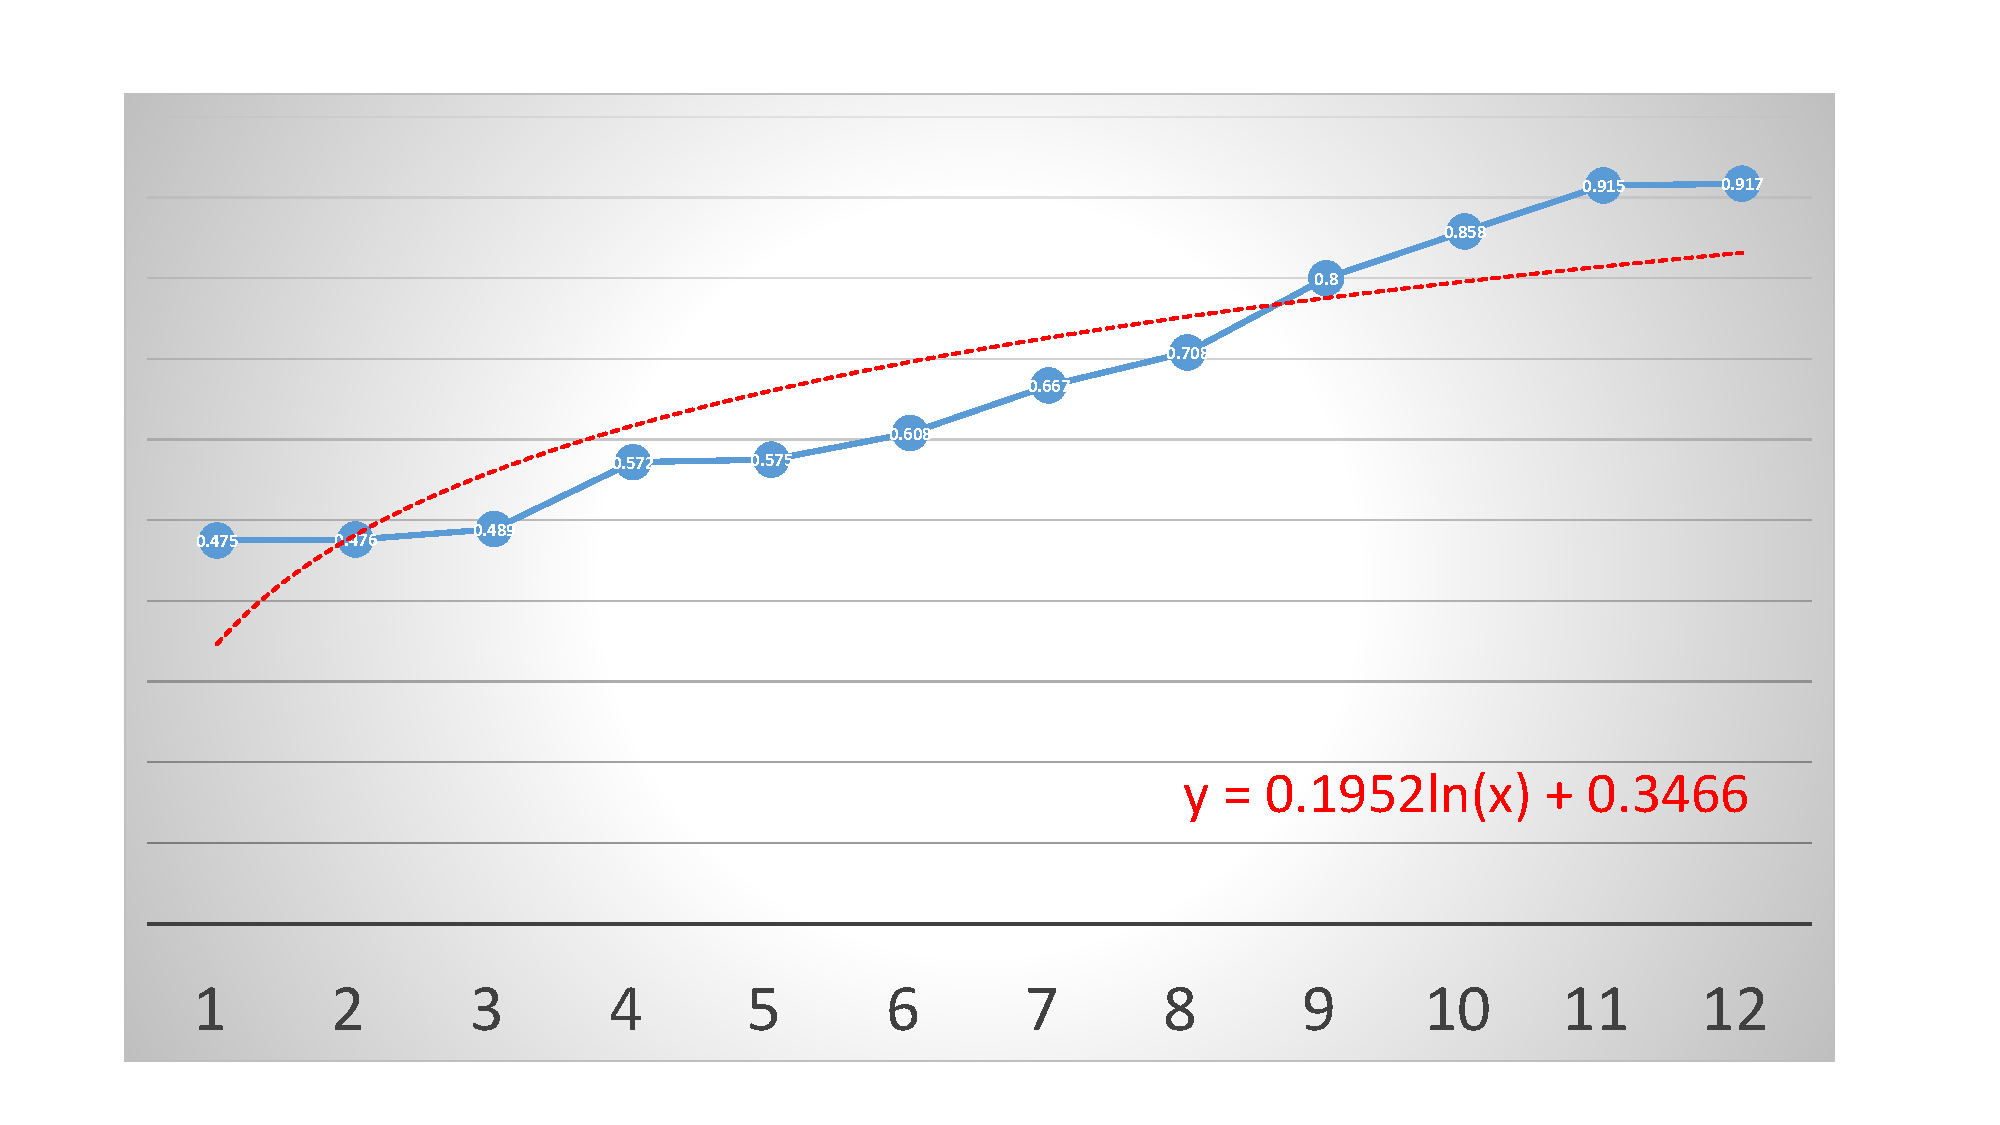
\includegraphics[width=15cm]{/figure/fig8.pdf}
\caption{The Yield-Time curve of remedial medicine for SARS, the regression result is used to describe our $\lambda$(Note that the temporal scale is month}\label{fig:8}
\end{figure}
We employee a logarithm function to regress the result. Therefore, our $\lambda$ is defined as:
\begin{equation}
\lambda \left( x,y,t+1\right) =0.195\ln \left( \dfrac{t}{30}\right) +0.35
\end{equation}

\subsubsection{S-R Transition Model}
The S-R transition probability $\eta(x,y,t)$ directly reflects the performance of vaccine medication. Apparently, for model simplification purpose, we utilize the \textbf{Assumption 2-5} like the P-R transition model again. However, the salient difference between P-R model and S-R model is that the speed of manufacturing a brand-new vaccine is much slower than that of remedial medicine. In this degree, the performance of the vaccine is determined as below by degrading the coefficients in some degree.
\begin{equation}
\eta \left( x,y,t+1\right) =0.080\ln \left( \dfrac{t}{30}\right) +0.1
\end{equation}
\subsubsection{Medication Demand and EWS Model}
Just as mentioned in previous sections, in our \textbf{SPARD} dispersal model, the medication is divided into two classes: vaccine and remedial drug. 
In the aspect of remedial drug demand, the situation is relatively easy to understand. The core principal is "How many sick, how much drug". Combining with \textbf{Assumption 2-1}, we only need to concentrate our attention on treating the "P" state patients and the \textbf{potential patients} before the next drug delivery period $T$(\textbf{Assumption 2-6}). Because the transition probability at time $t$ is $\tau$, and we have susceptible people $S(x,y,t)$, primary symptom people $P(x,y,t)$. We arrange the remedial drug amount by predicting there will be $\tau$ ratio people caught EVD in the next $T$ days. Thus, the demand for remedial drug $DEM_{r}(x,y,t)$ is given as below:
\begin{equation}
DEM_{r}(x,y,t)=S\left( x,y,t\right) \sum ^{T}_{i=0}\left( 1-\tau \right) ^{i}\tau 
\end{equation}
On the other hand, the vaccine plays an important role in controlling the trend of EVD dispersal by lowering the risk of people in a specific region to get caught the Ebola, i.e., lowering the value of $\tau$ and increase the value of $\eta$. Nevertheless, as we have deduced in S-P transition model, the probability of catching a EVD is not noly determined by the intra-district factors, but the neighbourhood regions, as well. On the basis of this assumption, we use the $DDI$ attribute and the "convolution integral" trick in S-P Transition Model again to calculate the demand for vaccine $DEM_{v}(x,y,t)$:
\begin{equation}
DEM_{v} \left( x,y,t\right) =\textbf{conv}\left[ DDI\left( x,y,t\right) ,F_{vacc}\left( x,y\right) \right]
\end{equation}
However, in this case, we abandon the classical two dimension Gaussian function  to conduct the convolution. 

\subsubsection{Transport Optimization}
\subsection{Experiment Result}
\subsection{Strengths and Weaknesses}

\section{Conclusion}

\bibliography{cites}
\begin{appendices}
\section{Codes}
%\subsection{Codes for sub-problem 1}
%\lstinputlisting[language=Matlab]{../code/script_UserAverScore.m}
%\subsection{Codes for sub-problem 2, 3}
%\lstinputlisting[language=Matlab]{../code/svm_regression_generator.m}
%\lstinputlisting[language=Matlab]{../code/svm_regression_generator.m}
\end{appendices}